
      \begin{animateinline}[final,loop,controls,poster=last]{1}
          \multiframe{8}{iCOUNT=00+01}{
      
  
  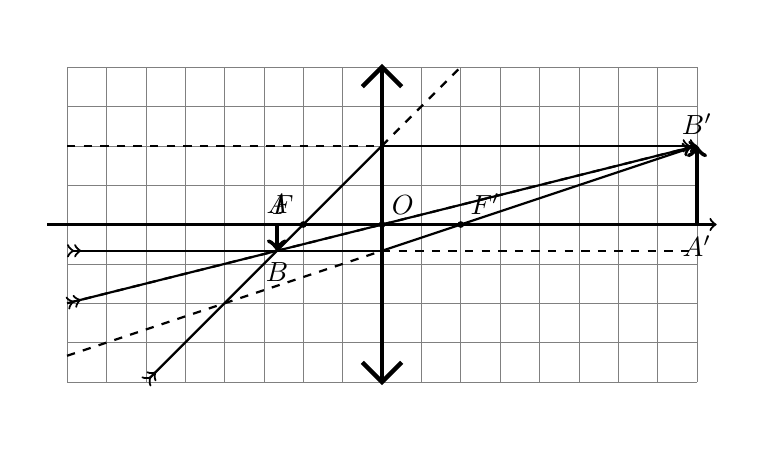
\begin{tikzpicture}[scale=0.5]
    \clip (-9,-5) rectangle (9,5) ;
    \draw [help lines] (-8,-4) grid [step=1] (8,4) ; %% Le quadrillage
    \draw [->,thick] (-8.5,0) -- (8.5,0) ; %% L'axe optique
    \draw [ultra thick] (0,-4) -- (0,4)  ; %% Le corps du systeme 

    % Dessin de la lentille et des points focaux
    \draw [ultra thick] (-0.5,-3.5) -- (0,-4) -- (0.5,-3.5)
                         (-0.5,3.5) -- (0, 4) -- (0.5,3.5) ;
    \filldraw [black] (2.0,0) circle (2pt) node [above right] {$F'$};
    \filldraw [black] (-2.0,0) circle (2pt) node [above left] {$F$} ;
    \filldraw [black] (0,0) circle (2pt) node [above right] {$O$} ;
    \ifthenelse{\iCOUNT > 6}{
      \draw [->,ultra thick] (-2.6666666666666665,0) node [above] {$A$} -- (-2.6666666666666665,-0.6666666666666666) node [below] {$B$} ;
      }{}

      \draw [->,ultra thick] (8.0,0) node [below] {$A'$} -- (8.0,2.0) node [above] {$B'$} ;
      % Le rayon qui arrive // a l'axe optique
\ifthenelse{\iCOUNT > 1}{
    \draw [thick ,>>-] (-8,-0.667) -- (0,-0.667);
    \draw [thick , dashed] (0,-0.667) -- (8,-0.667);
    }{}
% ... arrive en passant par le foyer image
\ifthenelse{\iCOUNT > 0}{
    \draw [thick , dashed] (-8,-3.333) -- (0,-0.667);
    \draw [thick ,->>] (0,-0.667) -- (8,2.0);
    }{}
% Le rayon qui passe par le centre optique
\ifthenelse{\iCOUNT > 3}{
    \draw [thick ,>>-] (-8,-2.0) -- (0,0.0);
    \draw [thick , dashed] (0,0.0) -- (8,2.0);
    }{}
% ... n'est pas devie
\ifthenelse{\iCOUNT > 2}{
    \draw [thick , dashed] (-8,-2.0) -- (0,0.0);
    \draw [thick ,->>] (0,0.0) -- (8,2.0);
    }{}
% Le rayon qui passe par le foyer objet
\ifthenelse{\iCOUNT > 5}{
    \draw [thick ,>>-] (-6.0,-4.0) -- (0,2.0);
    \draw [thick , dashed] (0,2.0) -- (2.0,4.0);
    }{}
% ... ressort // a l'axe optique
\ifthenelse{\iCOUNT > 4}{
    \draw [thick , dashed] (-8,2.0) -- (0,2.0);
    \draw [thick ,->>] (0,2.0) -- (8,2.0);
    }{}

  \end{tikzpicture}}
\end{animateinline}
